%%%%%%%%%%%%%%%%%%%%%%%%%%%%%%%%%%%%%%%%%%%%%%%%%%%%%
%%% Task 1 %%%%%%%%%%%%%%%%%%%%%%%%%%%%%%%%%%%%%%%%%%
%%%%%%%%%%%%%%%%%%%%%%%%%%%%%%%%%%%%%%%%%%%%%%%%%%%%%
\task{Fundamentals}

%%%%%%%%%%%%%%%%%%%%%%%%%%%%%%%%%%%%%%%%%%%%%%
\taskGerman{Grundlagen}

\begin{figure}[h!]
    \centering
    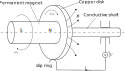
\includegraphics[width=0.6\textwidth]{fig/Faradays_disc.pdf}
    \caption{Faraday disk: Rotating copper disk in a magnetic field}
    \label{fig:faraday_disk}
\end{figure}



\subtask{The disc from Fig.~\ref{fig:faraday_disk} has a diameter of $d=\SI{60}{\cm}$ and is rotating with the circumferential speed $v_\mathrm{d} = \SI{100}{\meter\per\second}$. What is the rotational speed and angular velocity of the copper disk?}{2}
\subtaskGerman{Die Scheibe aus Abb.~\ref{fig:faraday_disk} hat einen Durchmesser von $d=\SI{60}{\cm}$ und ihre Oberfläche rotiert mit der Umfangsgeschwindigkeit $v_\mathrm{d} = \SI{100}{\meter\per\second}$. Wie groß ist die Drehzahl $n_\mathrm{d}$ und die Winkelgeschwindigkeit $\omega_\mathrm{d}$ der Kupferscheibe?}

\begin{solutionblock}
    The rotational speed is given by
    $$ n_\mathrm{d} = \frac{v_\mathrm{d}}{2\pi r} = \frac{\SI{100}{\meter\per\second}\cdot \SI{60}{\second\per\minute}}{2\pi \cdot \SI{0.3}{\meter}} = \SI{3183}{\per\minute}.$$
    The angular velocity is
    $$ \omega_\mathrm{d} = 2\pi n_\mathrm{d} \SI{\frac{1}{60}}{\minute\per\second} = \SI{333}{\per\second}.$$
\end{solutionblock}


\subtask{Assuming that the permanent magnet is not rotating ($\omega_\mathrm{r}=0$) while delivering a homogenous and constant magnetic field with $B=\SI{1.8}{\tesla}$, what is the measured induced voltage $U$?}{2}
\subtaskGerman{Angenommen, dass der Permanentmagnet nicht rotiert ($\omega_\mathrm{r}=0$) allerdings ein homogenes und konstantes Magnetfeld mit $B=\SI{1.8}{\tesla}$ liefert, wie groß ist die gemessene induzierte Spannung $U$?}

\begin{solutionblock}
    Faraday's law of induction reads 
    $$u_\mathrm{i} =\oint_{\partial\mathcal{S}} \bm{E} \cdot \mathrm{d}\bm{s}$$ 
    where $\bm{E}$ is the electric field and $\partial\mathcal{S}$ is the boundary of the surface $\mathcal{S}$, which is the copper disk in this case. The electric field is a resulting of the rotating magnetic field and points from the center to the edge of the disk along the radial direction:
    $$\bm{E} = \bm{v} \times \bm{B} = v(r) B \bm{e}_\mathrm{r} .$$
    Here, $\bm{v}(r) = 2 \pi r n_\mathrm{d}$ is the velocity field of the disk for a given radius element $r$ and $\bm{e}_\mathrm{r}$ is the unit vector in the radial direction. The induced voltage is then
    \begin{align*}
        u_\mathrm{i} &= \int_{0}^{d/2} v(r) B \mathrm{d}r = B \int_{r=0}^{d/2} 2 \pi r n_\mathrm{d} \mathrm{d}r = 2 \pi Bn_\mathrm{d} \left[\frac{r^2}{2}\right]_{0}^{d/2} = \pi B n_\mathrm{d} \frac{d^2}{4} = \pi \cdot \SI{1.8}{\tesla} \cdot \SI{53.05}{\per\second}\cdot \SI{0.09}{\meter} \\&= \SI{27}{\volt}.
    \end{align*}
\end{solutionblock}

\subtask{Sketech}{2}
\subtaskGerman{Skizziere}

